
This chapter covers the theoretical background for the research presented in this thesis. Starting with the description of the Standard Model, this chapter will analyze its limits and introduce one possible theoretical extension, supersymmetry. This additional theory can explain some of the phenomena in nature that the Standard Model cannot describe.

\section{Standard Model and the Higgs mechanism}

The Standard Model is a gauge theory with the gauge group $SU(3)_\mathrm{c} \otimes SU(2)_\mathrm{L} \otimes U(1)_Y$ in which color charge, weak isospin ($T_3$) , electric charge ($Q$), and weak hypercharge are conserved. This theory also describes three of the forces existing in nature, the electromagnetic, the weak and the strong force and defines the fundamental constituents of matter \cite{Spiesberger:2000ks}. It was developed in the second half of the twentieth century as combined theoretical and experimental effort by the research communities from all around the world. Since the first formulation at the beginning of the 1970s the Standard Model successfully predicted all the particles that were discovered later in the century. The most recent particle discoveries such as the top quark \cite{Campagnari:1996ai} (1995), the tauonic neutrino \cite{Agafonova:2015jxn} and finally the Higgs boson \cite{Aad:2012tfa,Chatrchyan:2012xdj}(2012) have given further credence to the Standard Model. 

According to this theoretical model the basic constituents of matter are the fermions, characterized by Fermi-Dirac statistics. Fermions include leptons and quarks, which are divided into three generations of identical structure and are of half integer spin. \autoref{table:fermions} shows all the fermions of the Standard Model and their charges, arranged in the three generations. Bosons are characterized by Bose-Einstein statistics and all have integer spins. Bosons may be either elementary, like photons and gluons, or composite, like mesons. Elementary bosons are responsible for the four fundamental forces of nature and are called force particles (gauge bosons). As shown in \autoref{table::bosons} the strong interaction is mediated by the gluon g, the weak interaction is mediated by the W and Z bosons, the electromagnetic force is mediated by the photon $\gamma$. 

\begin{figure}[tbh!]
	\begin{center}
		
		\begin{tabular}{ | c | c | c | c | c |}
			\hline
			& 1st Generation & 2 Generation & 3rd Generation & charge \\ \hline \hline
			& & & & \\
			leptons & $\left( \begin{array}{c} \nu_{e} \\ e \end{array} \right)_{\text{L}}$ & $\left( \begin{array}{c} \nu_{\mu} \\ \mu \end{array} \right)_{\text{L}}$ & $\left( \begin{array}{c} \nu_{\tau} \\ \tau \end{array} \right)_{\text{L}}$ & \begin{tabular}{@{}c@{}}weak \\ weak, electromagnetic\end{tabular} \\
			& & & & \\
			& $e_{\text{R}}$& $\mu_{\text{R}}$& $\tau_{\text{R}}$& electromagnetic\\ 
			& & & & \\
			\hline
			& & & & \\
			quarks & $\left( \begin{array}{c} u \\ d \end{array} \right)_{\text{L}}$ & $\left( \begin{array}{c} c \\ s \end{array} \right)_{\text{L}}$ & $\left( \begin{array}{c} t \\ b \end{array} \right)_{\text{L}}$ & weak, electromagnetic, strong \\
			& & & & \\
			& $u_{\text{R}}, d_{\text{R}}$& $c_{\text{R}}, s_{\text{R}}$& $t_{\text{R}}, b_{\text{R}}$& electromagnetic, strong\\
			& & & & \\ 
			\hline
			\hline
		\end{tabular}
		\caption{Fermions of the Standard Model and their charges, arranged in the three generations. Only the left-handed fermions interact weakly and are arranged in doublets. The right-handed fermions are singlets. The right-handed neutrinos are not present in this table, as they do not interact with one of the forces of the Standard Model.}
		\label{table:fermions}
	\end{center}
\end{figure}

\begin{table}
	%%%%%% SM BOSONS %%%%%%%
	\centering
	\begin{tabular}{| c || c | c | c | c | c |}
		\hline
		bosons & interaction & range [m] & spin $[\hbar]$ & $Q$ $[e]$ & mass [GeV/$c^2$]\\\hline\hline
		8 gluons &  strong  & $10^{-15}$ & 1 & 0 & 0 \\\hline
		$W^\pm$, $Z$ & weak  & $ 10^{-18}$ & 1 & $\pm 1$, 0 & $\approx$ 80.4, 91.2 \\\hline
		photon $\gamma$ &  electromagnetic  & $\infty$ & 1 & 0 & 0 \\\hline\hline
		higgs $h$ &  --  &  -- & 0 & 0 & $\approx 125$ \\\hline
		
	\end{tabular}
	\caption{
		The eleven gauge bosons or force carriers of the Standard Model and the corresponding force and force range, and the Higgs boson which breaks electroweak symmetry~\cite{pdg12}.
		The graviton, which is not included in the Standard Model and hence not included here, is a hypothetical spin-2, zero mass, zero electromagnetic charge, and infinite-range mediator of the gravitational force.
	}
	\label{table::bosons}
\end{table}

The electric charge $Q$ is the ganerator that the massless photon couples to. It is an invariant quantity and is defined as \cite{zee2003quantum}

\begin{equation}
Q = T_3 + \frac{1}{2}Y
\label{eqn:electricchargegenerator}
\end{equation}

Here $T$ denotes the generator of the isospin symmetry group $SU(2)$ and $Y$ denotes the generator of hypercharge symmetry group $U(1)_Y$. The $SU(2)$ generators obey the Lie algebra
\begin{equation}
[T^a, T^b] = i\varepsilon^{abc}T_c.
\label{eqn:su2liealgebr}
\end{equation}

where $\varepsilon^{abc}$ is the antisymmetric Levi-Civita symbol. Under the fundamental representation the generators of $SU(2)$  becomes the Pauli matrices: $T_a = \sigma_a/2$ \cite{roubillard2005th}. The Standard Model Langrangian is \cite{noteskooijman11}.

\begin{equation}
\mathcal L_{SM} = \mathcal L_{kinetic} + \mathcal L_{Higgs} + \mathcal L_{Yukawa},
\label{eqn:SMLagrangian}
\end{equation}
with the kinetic term describing the dynamics of the spinor fields $\psi$
\begin{equation}
\mathcal L_{kinetic} = i\overline{\psi}(\partial^\mu\gamma_\mu)\psi,
\label{eqn:SMLkinetic}
\end{equation}
with $\overline{\psi} \equiv \psi^\dag\gamma^0$, and $\psi$ the three fermion generations which will be later represented by an index $i$. 

The gauge invariance under the three symmetry group is imposed by replacing the derivative with a covariant derivative obtaining the fields of the interactions corresponding to the symmetry groups:

\begin{equation}
\mathcal L_{kinetic} =  i\overline{\psi}(D^\mu\gamma_\mu)\psi \\;
\label{eqn:newSMLkinetic}
\end{equation}
with
\begin{equation}
D^\mu = \partial^\mu + i\frac{g_s}{2}G^\mu_aL_a + i\frac{g}{2}W^\mu_b\sigma_b+i\frac{g'}{2}B^\mu Y,
\label{eqn:SMcovariant}
\end{equation}
where $L_a$ are the Gell-Mann matrices which gives the generators of $SU(3)$ so $t_a \equiv L_a/2$, $\sigma_b$ are the Pauli matrices which gives the generators of $SU(2)$ $T_a \equiv i\sigma_b/2$, $g_s$, $g$, and $g'$ are respectively the strong $SU(3)$, the electroweak isospin $SU(2)$, and hypercharge $U(1)$ couplings and $G^\mu_a$, $W^\mu_b$, and $B^\mu$ are respectively the eight gluon fields, the three weak interaction bosons that form a triplet, and the single hypercharge boson.

The fermion fields $\psi$ then transform as 
\begin{equation}
\psi(x) \to \mathrm{e}^{i\pi^a\sigma_a/2}\mathrm{e}^{iY\beta(x)}\psi(x),
\label{eqn:phitransformsagain}
\end{equation}
with $Y$ the generator of $U(1)$ and $\pi^a$ the parameters of the $SU(2)$ transformations. The abelian $U(1)_Y$ and the nonabelian $SU(2)_L$ have the Yang-Mills terms $\mathcal{L}_{gauge} = -\frac{1}{4}(G^a_{\mu\nu}G^{a\mu\nu} + H_{\mu\nu}H^{\mu\nu})$ with $H_{\mu\nu} = \partial_\mu B_{\nu} -\partial_\nu B_\mu$ and $G^a_{\mu\nu}= \partial_\mu W^a_\nu -\partial_\nu W^a_\mu + g\varepsilon^{abc}W^b_\mu W^c_\mu$, from which it can be seen that the gauge bosons self-interact \cite{roubillard2005th}.

The $SU(2)_L \times U(1)_Y$ gauge theory is the partially unified theory of the weak and electromagnetic interactions of Glashow, Weinberg, and Salam \cite{peskin1995introduction}. Through spontaneous breaking of the symmetry of these groups to $U(1)_{EM}$, the electromagnetic gauge group, the $W$ and $Z$ bosons gain mass. This works again according to the Higgs mechanism of the previous section; for this to occur, first a Higgs scalar field is to be added to the Lagrangian \cite{quigg1983gauge}:
\begin{equation}
\mathcal L_{Higgs} = (D_\mu\phi)^\dag(D^\mu\phi) - \mu^2\phi^\dag\phi - \lambda(\phi^\dag\phi)^2,
\label{eqn:SMLHiggs}
\end{equation}
from which the mass of the bosons comes from the interaction term (which contains a covariant derivative) after spontaneous symmetry breaking. This is a generalization of the abelian Higgs model to a nonabelian gauge group. Each fermion generation is made of five different representations \cite{peskin1995introduction}:

\begin{enumerate}
	\label{enum:hypercharges}
	\item Left-handed quarks $Q^I_{Li}$, which are a triplet under $SU(3)$, a doublet $\left(\begin{array}{c} u \\ d \end{array} \right)^I_{Li}$ under $SU(2)$, and have hypercharge $Y = \frac{1}{3}$;
	\item Right handed ``up'' quarks (i.e. up, charm, top)  $u^I_{Ri}$, which are an $SU(3)$ triplet, $SU(2)$ singlet, and have hypercharge $Y = \frac{4}{3}$;
	\item Right handed ``down'' quarks (i.e. down, strange, bottom)  $d^I_{Ri}$, which are an $SU(3)$ triplet, $SU(2)$ singlet, and have hypercharge $Y = \frac{-2}{3}$;
	\item Left-handed leptons  $L^I_{Li}$, which are an $SU(3)$ singlet, $SU(2)$ doublet  $\left(\begin{array}{c} \nu \\ e \end{array} \right)^I_{Li}$, and have hypercharge $Y = -1$;
	\item Right-handed ``electron'' leptons $L^I_{Ri}$, which are an $SU(3)$ singlet, $SU(2)$ singlet, and have hypercharge $Y = -2$. The name is given because only the electron, muon, and tau are included; right-handed neutrinos are not.
\end{enumerate}

Contrary to experimental evidence the mass of the right-handed neutrinos is comparable their lepton counterpart, therefore they have not been included in the list.

\subsection{The Bosonic Masses}
\label{section:bosonicmasses}
In the case $\phi(x)$  takes a vacuum expectation value of $v =  \sqrt{\frac{-\mu^2}{|\lambda|}}$, which corresponds to the minimum of the potential $V(\phi^\dag\phi) = \mu^2(\phi^\dag\phi) + |\lambda|(\phi^\dag\phi)^2$ only if $\mu^2<0$:

\begin{equation}
\left( \begin{array}{c}
\phi^+ \\
\phi^0 \end{array} \right) \rightarrow \frac{1}{\sqrt{2}}\left( \begin{array}{c}
0 \\
v \end{array} \right) \equiv \left<\phi\right>_0.
\label{eqn:vevphi}
\end{equation}

For this case , where $\left< 0 | \phi | 0\right> \neq 0$,  electroweak symmetry is spontaneously broken: $SU(2)_L\otimes U(1)_Y \to U(1)_{EM}$.
The generators of $SU(2)_L \otimes U(1)_Y$ do not leave this vacuum where v is assumed invariant. The generator corresponding to electric charge, however, does leave the vacuum invariant, so that the photon associated with electric charge will not acquire a mass \cite{quigg1983gauge}.

It is possible now to write $\phi$ in terms of fluctuations around its expectation value, as long as the original four degrees of freedom are retained:
\begin{equation}
\phi(x) = e^{i\frac{\boldsymbol{\vec{\xi}\cdot\overrightarrow{\sigma}}}{2}}\frac{1}{\sqrt{2}}\left( \begin{array}{c} 0 \\ v + h(x) \end{array} \right).
\label{eqn:phifluctuations}
\end{equation}
Now $\left<0|h(x)|\right> = 0$. Choosing the $U(1)$ gauge in such a way that the Lagrangian stays invariant, and using that $\phi(x)$ transforms as $\phi \rightarrow \phi' = U \phi$ with $U$ a unitary Hermitian matrix:
\begin{equation}
\phi \rightarrow \phi' =  e^{-i\frac{\boldsymbol{\vec{\xi}\cdot\vec{\sigma}}}{2}} \phi = \frac{1}{\sqrt{2}}\left( \begin{array}{c} 0 \\ v + h(x) \end{array} \right)
\label{eqn:trfmphigaugeU}
\end{equation}
where $h(x)$ is now the only degree of freedom remaining in this gauge \cite{roubillard2005th}. The gauge fields transform as
\begin{equation}
W^\mu_b\sigma_b \rightarrow W^{'\mu}_b\sigma_b \equiv  W^{\mu}_b\sigma_b; \hspace{5mm} B^\mu Y \rightarrow B^\mu Y.
\label{eqn:trfmWBbosons}
\end{equation}
Writing out the Higgs Lagrangian,
\begin{eqnarray}
\mathcal L_{Higgs} &=&  ((\partial_\mu + i\frac{g}{2}\sigma_bW_\mu^{'b} + i\frac{g'}{2}YB_\mu)\phi')^\dag \cdot (h.c.) + V(\phi^{'\dag}\phi') \nonumber \\
&&  \frac{1}{8}g'g \left( \begin{array}{cc} 0 & v + h(x) \end{array} \right) YB_\mu\sigma_aW^{\mu a} \left( \begin{array}{c} 0 \\ v + h(x) \end{array} \right) \nonumber \\
&& + \mbox{other interactions},
\label{eqn:LHiggsvaried}
\end{eqnarray}

the masses terms of the bosons are obtained from the squared terms. The $(W_\mu)^2$-term becomes:
\begin{eqnarray}
 \frac{1}{8}g^2 (v + h(x))^2 \left[\left(W_\mu^1\right)^2 + \left(W_\mu^2\right)^2 + \left(W_\mu^3\right)^2 \right], 
\label{eqn:Wsquaredterm}
\end{eqnarray}
Now the masses can be derived from the squared terms:
\begin{itemize}
	\item $\frac{1}{2}\mu^2h^2 \rightarrow h$ has mass $\mu$ (through self-interaction);
	\item $\frac{1}{8}g^{'2}Y^2v^2B_\mu B^\mu \rightarrow B_\mu$ has mass $\frac{g'v}{2}$ (since $Y_\phi =1$);
	\item $\frac{1}{8}g^2 v^2 \left[\left(W_\mu^1\right)^2 + \left(W_\mu^2\right)^2 + \left(W_\mu^3\right)^2 \right] \rightarrow W_\mu $ has mass $\frac{gv}{2}$.
\end{itemize}

However the observed bosons do not corresponds to the $W_\mu^a$ or $B_\mu$ particles. It is possible however to rearrange the Lagrangian so that the known $W_\mu^+$, $W_\mu^-$, $Z^0$, and $A_\mu$ (corresponding to the photon).

However, the particles that are actually observed are not the $W_\mu^a$ or $B_\mu$ particles. The definitions of the measurable particles, which are the $W_\mu^+$, $W_\mu^-$, $Z^0$, and $A_\mu$ (photon) can be found through rearranging the Lagrangian. The interaction term of $B_\mu$ and $W\mu$ is 
\begin{equation}
-\frac{1}{4}(v+h)^2 g'g B_\mu W^{\mu 3},
\label{eqn:WBinteraction}
\end{equation}
so that, combining equations \ref{eqn:LHiggsvaried}, \ref{eqn:Wsquaredterm}, and \ref{eqn:WBinteraction},
\begin{eqnarray}
\mathcal L_{Higgs} &=&  \frac{1}{2}\partial_\mu h \partial^\mu h + \frac{1}{8}g^{'2}Y^2B_\mu^2(v+h)^2 + \frac{1}{2}\mu^2(v + h)^2 + \frac{1}{4}|\lambda|(v+h)^4 \nonumber \\
&\equiv& -\frac{1}{2}\mu^2h^2 + \frac{v^2}{8}\left[2g^2(W_\mu^+W_\mu^-) + (g^{'2} +g^2)Z_\mu^2 \right] + \nonumber \\
&& \mbox{other interactions}.
\label{eqn:Lredefined}
\end{eqnarray}
From this we can define the observable bosons:
\begin{eqnarray}
W^\pm_\mu &=&  \frac{W_\mu^1 \mp iW_\mu^2}{\sqrt{2}};\\
Z_\mu^0 &=& \frac{-g'B_\mu + gW_\mu^3}{\sqrt{g^2+g^{'2}}};\\
A_\mu &=&  \frac{gB_\mu + g'W_\mu^3}{\sqrt{g^2+g^{'2}}}.
\label{eqn:realbosonsdefined}
\end{eqnarray}
The zero in $Z_\mu^0$ underlines the fact that it is a neutral boson, as opposed to the charged $W^\pm_\mu$ bosons. The masses of the $W$ and $Z$ bosons finally becomes: $m_W = \frac{gv}{2}$ and $m_Z = \sqrt{g^2 + g^{'2}}\frac{v}{2} \equiv \frac{m_W}{\cos\theta_W}$. The term $\theta_W$ is known as the mixing angle; it is so called because it denotes the mixing of the $W$ and $B$ bosons that are composites of the $Z$ and $A$ bosons. The mixing angle $\theta_W$ is defined as follows:
\begin{eqnarray}
\cos\theta_W = \frac{g}{\sqrt{g^2 + g^{'2}}}, \hspace{2mm} \sin\theta_W = \frac{g'}{\sqrt{g^2 + g^{'2}}}.
\label{eqn:mixingangle}
\end{eqnarray}
The relationships between the $W$ and $B$ and $Z$ and $A$ bosons are then
\begin{equation}
\left( \begin{array}{c} Z^0 \\ A_\mu \end{array} \right) = \left( \begin{array}{cc} \cos \theta_W & -\sin \theta_W \\ \sin\theta_W & \cos\theta_W \end{array} \right) \left( \begin{array} {c} W^3_\mu \\ B_\mu \end{array} \right);
\label{eqn:ZAWBmixing}
\end{equation}

\subsection{The couplings $g$ and $g'$}

The coupling constants $g$ and $g'$ are derived from the interaction term between the $A_\mu$ boson and a lepton in $\mathcal L_{kinetic}$ from equations \ref{eqn:newSMLkinetic} and \ref{eqn:SMcovariant}, using the definition of $A_\mu$ from equation \ref{eqn:realbosonsdefined}, and using $L_L \equiv \left( \begin{array}{cc} \nu \\ e \end{array}\right)_L$ and $L_R \equiv e_R$. In the case of the electron:
\begin{eqnarray}
\mathcal L_{A_\mu-electron} &=&  \overline{e}_R\gamma^\mu g' \frac{g}{\sqrt{g^2 + g^{'2}}} A_\mu e_R + \overline{e}_L\gamma^\mu \frac{g'}{2} \frac{g}{\sqrt{g^2 + g^{'2}}} A_\mu e_L + \nonumber \\
&=&  \frac{gg'}{\sqrt{g^2 + g^{'2}}}\bar{e}\gamma_\mu e A^\mu .\\
\label{eqn:ALinteraction}
\end{eqnarray}
Identifying $A_\mu$ as the photon, it is possible to set the coupling $ e \equiv \frac{gg'}{\sqrt{g^2 + g^{'2}}}$. 

\subsection{Fermion Masses}
\label{section:fermionmasses}

In order to generate the other fermion masses an interaction between the scalar field $\phi(x)$ and the fermions is needed. The best choice is the interaction of $\phi(x)$ with fermions given by the Yukawa coupling \cite{noteskooijman11} which does obey the necessary symmetries of $SU(3)_C \otimes SU(2)_L \otimes U(1)_H$:
\begin{eqnarray}
\mathcal L_{Yukawa} &=& Y_{ij}\overline{\psi_{i}}\phi\psi_{j}\\
\label{eqn:SMLYukawa}
\end{eqnarray}
where $Y$ is the Yukawa coupling constant, and $i$,$j$ are flavor indices that matter for QCD.
In order for this Lagrangian to be Lorentz invariant, $\phi(x)$is chosen as in \autoref{eqn:phifluctuations} and it transforms as in \autoref{eqn:trfmphigaugeU}. The fermion field transforms as $\psi \rightarrow \psi' = e^{-i\frac{\boldsymbol{\vec{\xi}\cdot\vec{\sigma}}}{2}} \psi$. Then the transformation of the term with the $d$-quark will be as follows:
\begin{eqnarray}
\mathcal L_{Yukawa,quarks,d_R}' &=&  Y^d_{ij}\overline{Q^{I'}_{Li}}\phi' d^{I'}_{Rj} + h.c. \nonumber \\
&=& Y^d_{ij}  \left( \overline{ \begin{array}{cc} u & d \end{array} } \right)^I_{Li}  \frac{1}{\sqrt{2}} \left( \begin{array}{c} 0 \\ v + h(x)\end{array} \right)  d^I_{Rj} + h.c.\nonumber \\
\mathcal L_{Yukawa,d-quark} &=&  Y^d_{ij}   \overline{d}^I_{Li} \frac{v}{\sqrt{2}} d^I_{Rj}  + h.c. + \mbox{interaction terms} \nonumber \\
&=& M^d_{ij}\overline{d}^I_{Li}d^I_{Rj} + h.c. + \mbox{interaction terms}.
\label{eqn:SMLYukawaDquark}
\end{eqnarray}
The mass terms can be derived from the diagonal form of the mass matrix $M^d_{ij}$. This diagonal form is obtained with the usage of the unitary matrices $V^d$ which obey the following rules:
\begin{eqnarray}
V_L^{d\dag}V_L^d &=&  1,\\
(V^d_R)_{ij}d^I_{Rj} &\equiv& d_{Ri}, \\
\overline{d}_{Li}^I (V_L^{d\dag})_{ij} &\equiv& \overline{d}_{Lj}, \\
V^{d}_L M^d V^{d\dag}_R &=&  M^d_{diag},
\label{eqn:diagonalizingMmatrix}
\end{eqnarray}
with $d_L$ and $d_R$ the down quark in its mass eigenstate. This gives
\begin{eqnarray}
\mathcal{L}_{Yukawa,d-quark} &=& M^d_{ij}\overline{d}^I_{Li}M^d_{ij}d^I_{Rj} + h.c. + \mbox{interaction terms} \nonumber \\
&=& \overline{d}_{Li}V^{d\dag}_LV^d_L(M^d_{ij})V^{d\dag}_R V^d_Rd^I_{Rj} + h.c. + \mbox{interaction terms} \nonumber \\
&=& \overline{d}_{Li}(M^d_{ij})_{diag}d_{Rj} + h.c. + \mbox{interaction terms}.
\label{eqn:SMLYukawaDquarkMassEigenstates}
\end{eqnarray}
The down quark has finally acquired mass. In order to obtain the mass of the up quark a new definition of the spinor $\phi$ is needed:

\begin{eqnarray}
\tilde{\phi} &=&  i\sigma_2\phi^* \nonumber \\
&=&  i \left( \begin{array}{cc} 0 & -i \\ i & 0 \end{array} \right)  \left( \begin{array}{c} \phi^{+*} \\ (\phi^{0})^* \end{array} \right) \nonumber \\
&=&  \left( \begin{array}{cc} 0 & 1 \\ -1 & 0 \end{array} \right)  \left( \begin{array}{c} \phi^{+*} \\ (\phi^{0})^* \end{array} \right) \nonumber \\
&=&   \left( \begin{array}{c} (\phi^0)^* \\ -(\phi^+)^* \end{array} \right).
\label{eqn:SMphitilde}
\end{eqnarray}
which gives the proper term in the Yukawa potential. Furthermore $\tilde{\phi}$ is a Lorentz scalar and transforms in the same way as $\phi$ did: 

\begin{eqnarray}
\tilde{\phi} = i\sigma_2\phi^* &\rightarrow& i\sigma_2\left(e^{\frac{i}{2}\vec{\xi} \cdot \vec{\sigma}} \phi \right)^* \nonumber \\
&\approx& e^{\frac{i}{2}\vec{\xi} \cdot \vec{\sigma}} \tilde{\phi},
\label{eqn:trmfphitilde}
\end{eqnarray}
 $\tilde{\phi}$ can be redefined as:
\begin{equation}
\tilde{\phi} = e^{\frac{i}{2}\mathbf{\xi \cdot \sigma}}\left( \begin{array}{c} v+h \\ 0 \end{array} \right)
\label{eqn:phitildedefined}
\end{equation}
where the vacuum expectation value of $\tilde{\phi}$ has been used:
\begin{equation}
\left<\tilde{\phi}\right>_0 = \left<i\sigma_2\phi^*\right>_0 = \frac{1}{\sqrt{2}} \left( \begin{array}{c} (v + h)^* \\ 0 \end{array} \right) = \frac{1}{\sqrt{2}} \left( \begin{array}{c} v + h \\ 0 \end{array} \right)
\label{eqn:vevphitilde}
\end{equation}
the up quark term of the Yukawa potential finally becomes:
\begin{eqnarray}
\mathcal L_{Yukawa,quarks,u} &=&  Y^u_{ij}\overline{Q^I_{Li}}\tilde{\phi} u^I_{Rj} + h.c. \nonumber \\
&=& Y^d_{ij}  \left( \overline{ \begin{array}{cc} u & d \end{array} } \right)^I_{Li}  \frac{1}{\sqrt{2}}  \left( \begin{array}{c} v + h \\ 0 \end{array} \right)  u_{Rj} + h.c.\nonumber \\ 
&=& \overline{u}^I_{Li}M^u_{ij}u^I_{Rj} + h.c. + \mbox{interaction terms} \nonumber \\
&=& \overline{u}^I_{Li}V^{u\dag}_LV^u_L(M^u_{ij})V^{u\dag}_R V^u_Ru^I_{Rj} + h.c. + \mbox{interaction terms} \nonumber\\
&=& \overline{u}_{Li}(M^u_{ij})_{diag}u_{Rj} + h.c. + \mbox{interaction terms};
\label{eqn:SMLYukawaUquark}
\end{eqnarray}
and the up quark has acquired a mass.

\subsection{Standard Model limitations}

Over the decades the Standard Model has been successful in predicting existence of particles and their properties at the electroweak scale. However several questions remain open:

\begin{itemize}
	\item The Standard Model does not include gravity, therefore it cannot be a complete description of nature;
	\item Although the representation of the strong and electroweak force by $SU(2)_L\otimes U(1)_Y \to U(1)_{EM}$ is successful, the Standard Model does not have the unification of the force coupling constants at the Planck scale.
	\item Astrophysical observations gives evidence to the existence of a much greater amount of matter in the universe that can be explained by baryonic matter \cite{deBoer:2005tm}, known also under the name of \textit{dark matter}. There are theoretical models that associates the Standard Model neutrinos with "hot Dark Matter" \cite{Klypin:1992sf}, however experimental observations are more consistent with  "cold Dark Matter" models which have a non-Standard Model particle candidate \cite{Jungman:1995df}.
	\item Neutrinos are considered massless in the Standard Model. Recent experiments proved that neutrinos have masses \cite{Fukuda:1998mi};
	\item In the Standard Model, the quantum corrections to the Higgs mass are quadratically divergent. Starting from the assumption that every form of interaction possible by a particle will happen and will contribute to the total mass of the particle, the mass of the Higgs boson is 
	
	\begin{equation}
	\mu^{2}_{\text{eff}} = \mu^{2}_{0} + \delta\mu^{2}_{0} \approx 125\gev
	\end{equation}
	
	where $\mu^{2}_{0}$ is the bare mass of the particle, and $\delta\mu^{2}_{0} $ is its total correction. Taking into account the assumption that Standard Model is correct up to the Plank scale, the total correction would be of the order  $\delta\mu^{2}_{0}  \sim \Lambda^{2} \sim M^{2}_{\text{Planck}} \sim 10^{28}M^{2}_{\text{EW}}$ resulting in a very heavy Higgs Boson. These assumptions are in contrast with the discovery of the Higgs boson with an invariant mass around 125\gev by the experiments ATLAS \cite{Aad:2012tfa} and CMS \cite{Chatrchyan:2012xdj} giving raise to the so-called \textit{Hierarchy Problem}.
	
\end{itemize}

\clearpage



This chapter summarizes the theoretical background for the research presented in this thesis. Starting with the description of the Standard Model,  limitations and one possible theoretical extension, supersymmetry, is introduced. This theory can explain some of the phenomena in nature that the Standard Model cannot describe.

\section{Supersymmetry}

Supersymmetry is one of the most intriguing and fundamental concepts in modern theoretical particle physics. It arises naturally from the combination of the two cornerstones of 20th century physics: quantum field theory \cite{Miller:2013jra}. Supersymmetry is the unique symmetry that relates the two fundamental kinds of particles: bosons, which act as the carriers of forces, and fermions, which act as the constituents of matter. Supersymmetric quantum field theories have very special, improved properties, compared to ordinary relativistic quantum field theories. If supersymmetry is realized in nature, every fermion in the SM must have a bosonic partner particle. No such superpartner particle has been observed so far but there are more and more indications that these particles might show up at the LHC experiments \cite{Athron:2011wu}.

The most important aspect of superymmetry is the tranformation that turns a bosonic state into a fermionic state, and vice versa. The operator responsible for the transformation \textit{Q} must be an anti-commuting spinor with:

\begin{equation}
Q\left|\text{Bosons}\right> = \left|\text{Fermions}\right>, \quad Q\left|\text{Fermions}\right> = \left|\text{Bosons}\right>. 
\end{equation}

Suupersymmetry is defined as a space-time symmetry given that the $Q$ and $Q^{\dagger}$ are able to carry over spin and angular momentum. As a realistic theory with right- and left-handed fermions the transformation generators must fulfill the following commutation and anti-commutation rules:

\begin{equation}
\begin{array}{l c l}
\left\{Q, Q\right\} = P_{\mu}, \\
\left\{Q, Q\right\} = \left\{Q^{\dagger}, Q^{\dagger}\right\} = 0, \\
\left[P_{\mu}, Q\right] = \left[P_{\mu}, Q^{\dagger}\right] = 0,
\end{array}
\end{equation}

where $P_{\mu}$ is the generator of space-time translations. The single-particle states of a supersymmetric theory fall into irreducible representations of the supersymmetry algebra, called supermultiplets. Each of the supermultiplets contains both fermions and bosons, know as each other \textit{superpartners}. Given the members of the same multiplets $\left|\Omega\right>$ and $\left|\Omega^{\prime}\right>$, $\left|\Omega^{\prime}\right>$ is a combination of the operators $Q$ and $Q^{\dagger}$ acting on $\left|\Omega\right>$ and is invariant under space-time translation and rotation transformation \cite{Martin:1997ns}. Another important property of the generators $Q$ and $Q^{\dagger}$ is the commutation features with the squared mass operator $-P^{2}$, which translates into the same eigenvalues of the $-P^{2}$ operator shared among of the particles of the supermultiplets, therefore the supersymmetric particle shares same mass values as the original particle. Finally the supersimmetric generator commutes with the gauge transformation generators, therefore each of the Standard model particle and its superpartner have the same electric charges, weak isospin, and color degrees of freedom.
Each supermultiplet also contains an equal number of fermion and boson degrees of freedom \cite{Martin:1997ns}.

\subsection{Particle content}

\FloatBarrier

In the supersymmetric extension of the Standard Model each of the known fundamental particles belongs to a chiral or gauge multiplet, and has a superpartner with spin differing by $1/2$. The way particles fit into multiplets starts with observing that only chiral supemultiplets can contain fermions for the reason that their left-handed parts transform differently under the gauge group rules than their right-handed parts. All of the Standard Model fermions have those transformation properties, therefore they are members of chiral supermultiplets. On the other hand their superpartners must be spin 0 and not spin 1 vector bosons \cite{Martin:1997ns}.

The names for the spin-0 superpartners are constructed by adding the letter \textit{s}, as scalar, at the beginning of the fermion names. So generically they are called squark and sleptons (short form for \textit{scalar quark} and \textit{scalar lepton}). As in the Standard Model each of the two-component Weyl fermions has its own scalar partner. The symbol convention for squarks and sleptons is the same as the corresponding fermion with the addition of the tilde ($\sim$) symbol, e.g. $\widetilde{e}$ for the selectron. It is very important to denote that a sfermion given "handedness" does not refer to its helicity, being a spin-0 particle, but to its superparner helicity. A similar nomenclature is applied to smuons and staus: $\widetilde{\mu}_{L}$, $\widetilde{\mu}_{R}$, $\widetilde{\tau}_{L}$, $\widetilde{\tau}_{R}$. The Standard Model neutrinos are always left-handed and their superpartners are generically denoted as $\widetilde{\nu}$. The gauge interactions of squarks and sleptons are the same as for the corresponding Standard Model fermions; for instance the left handed squarks $\widetilde{u}_{L}$ and $\widetilde{d}_{L}$ couple to the W bosons, while $\widetilde{u}_{R}$ and $\widetilde{d}_{R}$ don't.

The Higgs boson is a spin-0 particle, so it must reside in a chiral supermultiplet. However, with the presence of a single Higgs boson in the supermultiplet the electroweak gauge symmetry would suffer a gauge anomaly, and would be inconsistent as a quantum theory. The conditions for the cancellations of this anomaly include the matrix trace $\text{Tr}[\text{T}^{2}_{3}\text{Y}] = \text{Tr}[\text{Y}_{3}] = 0$, where $\text{T}_{3}$ and Y are the third component of weak isospin and the weak hypercharge, respectively, in a normalization where the ordinary electric charge is $Q = T_{3} + Y$ . The traces run over all of the left-handed Weyl fermionic degrees of freedom in the theory. In the Standard Model, these conditions are already satisfied by the known quarks and leptons. The fermionic partner of a Higgs chiral supermultiplet has to be a weak isodoublet with weak hypercharge of $Y = \pm 1/2$. In both case such fermion would give a non-zero contribution to the traces and consequently spoil the anomaly cancellation. This can however be avoided by imposing two higgs supermultiplets, one with each of $Y = \pm1/2$, so that they cancel each other's contribution to the traces out. Another reason to justify the existence of two Higgs boson chiral multiplets is the structure of the supersymmetric theory itself: only the $Y = -1/2$ Higgs chiral supermultiplet can have the Yukawa couplings necessary to give masses to charge $+2/3$ up-type quarks (up, charm, top), and only a $Y = -1/2$ Higgs can have the Yukawa couplings necessary to give masses to charge $-1/3$ down-type quarks (down, strange, bottom) and to the charged leptons. 

The $\text{SU}(2)_{L}$ scalar fields are defined as $\text{H}_{u}(Y = +1/2)$ and $\text{H}_{d}(Y = -1/2)$. The weak isospin components of $\text{H}_{u}$ with $T_{3} = (1/2, -1/2)$ have electric charges 1 and 0 respectively, and are denoted ($\text{H}^{+}_{u}$, $\text{H}^{0}_{u}$). Similarly, the remaining doublet $\text{H}_{d}$ has $T_{3} = (1/2, -1/2)$ components ($\text{H}^{0}_{d}$, $\text{H}^{-}_{d}$). The Standard Model Higgs is a linear combination of $\text{H}^{0}_{u}$ and $\text{H}^{0}_{d}$. The standard nomenclature for a spin 1/2 superpartner is to add the suffix "-ino" to the name of the original Standard Model particle, e.g. the fermionic partners of the Higgs Scalars are called higgsinos. They are defined as $\widetilde{H}_{u}$, $\widetilde{H}_{d}$ for the $\text{SU}(2)_{\text{L}}$-doublet left-handed Weyl spinor fields, with weak isospin components $\widetilde{H}^{+}_{u}$,$\widetilde{H}^{0}_{u}$ and $H^{0}_{d}$,$\widetilde{H}^{-}_{d}$.

All the chiral multiplets are summarized in Table \ref{fig:chiral_supermultiplet}, classified according to their transformation properties under the Standard Model gauge group $\text{SU}(3)_{C} \times \text{SU}(2)_{L} \times \text{U}(1)_{Y}$.

\begin{table}[tbh!]
	\centering
	\begin{tabular}{|c || c | c | c | c |}
		\hline
		\multicolumn{2}{|c|}{chiral supermultiplets} & spin 0 & spin 1/2 & $\mathrm{SU}(3)_{\mathrm{c}}$, $\mathrm{SU}(3)_{\mathrm{L}}$, $\mathrm{U}(1)_{\mathrm{Y}}$\\\hline\hline
		\multirow{3}{*}{squarks, quarks (3 families)} &  $Q$  & ($\widetilde{u}_{\mathrm{L}}$, $\widetilde{d}_{\mathrm{L}}$) & ($u_{\mathrm{L}}$, $d_{\mathrm{L}}$) & $\mathbf{3}$, $\mathbf{2}$, 1/3 \\
		& $\bar{u}$ & $\widetilde{\bar{u}}_{\mathrm{L}}$ ($\widetilde{u}_{\mathrm{R}}^*$) & $\bar{u}_{\mathrm{L}} \sim (u_{\mathrm{R}})_{\mathrm{c}}$ & $\bar{\mathbf{{3}}}$, $\mathbf{1}$, -4/3 \\
		& $\bar{d}$ & $\widetilde{\bar{d}}_{\mathrm{L}}$ ($\widetilde{d}_{\mathrm{R}}^*$) & $\bar{d}_{\mathrm{L}} \sim (d_{\mathrm{R}})_{\mathrm{c}}$ & $\bar{\mathbf{3}}$, $\mathbf{1}$, 2/3 \\\hline
		\multirow{2}{*}{sleptons (3 families)} & $L$ & ($\widetilde{\nu}_{e\mathrm{L}}$, $\widetilde{e}_{\mathrm{L}}$) & ($\nu_{\mathrm{L}}$, $e_{\mathrm{L}}$) & $\mathbf{1}$, $\mathbf{2}$, -1 \\
		& $\bar{e}$ & $\widetilde{\bar{e}}_{\mathrm{L}}$ ($\widetilde{e}_{\mathrm{R}}^*$) & $\bar{e}_{\mathrm{L}} \sim (e_{\mathrm{R}})_{\mathrm{c}}$& $\mathbf{1}$, $\mathbf{1}$, 2 \\\hline
		\multirow{2}{*}{higgs, higgsinos} & $H_{\text{u}}$ & $\left(H_{\text{u}}^+,~H_{\text{u}}^0\right)$ & $\left(\widetilde{H}_{\text{u}}^+,~ \widetilde{H}_{\text{u}}^0\right)$ & $\mathbf{1}$, $\mathbf{2}$, 1 \\
		& $H_{\text{d}}$ & $\left(H_{\text{d}}^0,~H_{\text{d}}^-\right)$ & $\left(\widetilde{H}_{\text{d}}^0,~ \widetilde{H}_{\text{d}}^-\right)$ & $\mathbf{1}$, $\mathbf{2}$, -1 \\\hline
	\end{tabular}
	\caption{Chiral supermultiplets in the Minimal Supersymmetric Standard Model. The spin-0
		fields are complex scalars, and the spin-1/2 fields are left-handed two-component Weyl fermions.}
	\label{fig:chiral_supermultiplet}
\end{table}

The vector bosons of the Standard Model belong to the so called gauge multiplets. Their fermionic superpartners are called gauginos. In the Standard Model the color gauge interactions are mediated by the gluon g, whose spin-1/2 superpartner is the gluino $\widetilde{g}$. The electroweak symmetry breaking is associated with the $\text{W}^{\pm}$, $\text{W}^{0}$ and $\text{B}^{0}$ bosons, whose superparters are the winos $\widetilde{\text{W}}^{\pm}$, $\widetilde{\text{W}}^{0}$ and bino $\widetilde{\text{B}}^{0}$. After the symmetry breaking the Z boson and the photon $\gamma$ are given as mix of the $\text{W}^{0}$ and $\text{B}^{0}$ mass eigenstates. 

 Table \ref{fig:gauge_supermultiplets} summarizes the gauge supermultiplets of a minimal supersymmetric extension of the Standard Model, the Z boson and the photon $\gamma$ are given as mix of the $\text{W}^{0}$ and $\text{B}^{0}$ mass eigenstates \cite{PhysRevD.13.974}, also the SUSY gauge boson mix. From the mixing of the neutral gauginos $\widetilde{\text{W}}^{0}$ and $\widetilde{\text{B}}^{0}$ and higgsinos $H^{0}_{u}$ and $H^{0}_{d}$ come the four neutralinos $\widetilde{\chi}^{0}_{i}$ with $i \in 1,2,3,4$. Neutralinos couples to the gauge bosons, allowing for example a neutralino pair production through Drell-Yan processes. The mixing of the charged gauge bosons $\widetilde{\text{W}}^{\pm}$ and higgsinos $\widetilde{H}^{+}_{u}$ and $\widetilde{H}^{-}_{d}$ creates the four charginos $\widetilde{\chi}^{+}_{i}$ and $\widetilde{\chi}^{-}_{i}$. Because these particles are mixed states of other particles, if a particle is dominantly one of the states, one could call it “like” that particle state. For example, a second neutralino can be “winolike” if its mixed state comes mostly from the wino. “Bino-like” and “higgsino-like” describe similar situations for particles consisting of mixed states that are largely bino and higgsino, respectively.

\begin{table}[tbh!]
\centering
\begin{tabular}{|c || c | c | c |}
	\hline
	gauge supermultiplets & spin 1/2 & spin 1 & $\mathrm{SU}(3)_{\mathrm{c}}$, $\mathrm{SU}(3)_{\mathrm{L}}$, $\mathrm{U}(1)_{\mathrm{Y}}$\\\hline\hline
	gluinos, gluons & $\widetilde{g}$ & $g$ & $\mathbf{8}$, $\mathbf{1}$, 0\\\hline
	winos, $W$ bosons & $\widetilde{W}^\pm$, $\widetilde{W}^0$ & $W^\pm$, $W^0$ &   $\mathbf{1}$, $\mathbf{3}$, 0\\\hline
	bino, $B$ boson & $\widetilde{B}$ & $B$ &   $\mathbf{1}$, $\mathbf{1}$, 0\\\hline
\end{tabular}
	\caption{Gauge supermultiplets in the Minimal Supersymmetric Standard Model.}
	\label{fig:gauge_supermultiplets}
\end{table}

\FloatBarrier

\subsection{The MSSM}

\FloatBarrier

The chiral and gauge supermultiplets in Tables \ref{fig:chiral_supermultiplet} and \ref{fig:gauge_supermultiplets} constitute the particle content of a model of SUSY called Minimal Supersymmetric Standard Model (MSSM). Up to now none of the superpartners of the Standard Model has been discovered. If supersymmety were unbroken, then all the sparticles would be extremely easy to detect; there would have to be for example selectrons with masses exactly equal to the electron mass. A similar statement can be applied to all the others superpatners of the known Standard Model particles. The experimental evidence collected so far shows clearly that supersymmetry a broken symmetry in the vacuum state chosen by Nature \cite{Martin:1997ns}.

Supersymmetry can be broken by introducing extra terms into the Lagrangian that explicitly break the symmetry. A way to break supersymmetry is defined as \textit{soft} \cite{Dimopoulos:1981zb}: the extra terms should be of positive mass dimension in order to maintain naturally a hierarchy between the electroweak scale and the Planck scale \cite{Martin:1997ns}. Soft also means the theory is still renormalizable and the cancellation of quadratic divergences is preserved. One of the possible Lagrangian terms that could break supersymmetry is the quadratic term in the scalar field $\phi$ \cite{Martin:1997ns}.

The MSSM is often characterized by the choice of a superpotential which includes all the gauge invariants and renormalizable term, but on the other hand takes into account the softly broken supersimmetry and the conservation of the R-parity. The R-parity of a particle is imposed in order to justify the stability of the proton \cite{Martin:1997ns} and is defined as:

\begin{equation}
P_{R} = (-1)^{3(B-L)+2s}
\end{equation}

where \textit{B}, \textit{L} and \textit{s} are the particle baryonic,  lepton number and spin respectively. 

Is it possible to rewrite the scalar potential for the MSSM using the Higgs doublets\cite{Martin:1997ns}:

\begin{equation}
W_{\mathrm{MSSM}} = \bar{u}\mathbf{y_u}QH_u - \bar{d}\mathbf{y_d}QH_d - \bar{e}\mathbf{y_e}LH_d + \mu H_uH_d.
\label{eq::mssmpotential}
\end{equation}
The object $Q$ contains the left-handed squark and quark doublets, whereas the objects $\bar{u}$ and $\bar{d}$ contain $\widetilde{u}^*_{\text{R}}$, ${u}^\dag_{\text{R}}$ and $\widetilde{d}^*_{\text{R}}$, ${d}^\dag_{\text{R}}$, respectively. Similarly $L$ and $\bar{e}$ contain the slepton and lepton SU(2)$_{\mathrm{L}}$ doublets and singlets, respectively. The Yukawa matrices $\mathbf{y_u}$, $\mathbf{y_d}$, and $\mathbf{y_e}$ are dimensionless coupling parameters in the family space.

The symmetry breaking is exclusively coming from the soft SUSY-breaking terms \cite{Martin:1997ns}. The soft MSSM Lagrangian $\mathcal{L}_{\mathrm{soft}}^{\mathrm{MSSM}}$ is built combining the MSSM superpotential shown in \autoref{eq::mssmpotential} with the soft breaking terms and finally the kinetic mass terms\cite{Martin:1997ns}:

\begin{eqnarray}
\mathcal{L}_{\mathrm{soft}}^{\mathrm{MSSM}} &=& -\frac{1}{2}\left(M_3\widetilde{g}\widetilde{g} + M_2 \widetilde{W}\widetilde{W} + M_1\widetilde{B}\widetilde{B} + \mathrm{c.c.}\right)\nonumber\\
& & -\left(\widetilde{\bar{u}}\mathbf{a_u}\widetilde{Q}H_u - \widetilde{\bar{d}}\mathbf{a_d}\widetilde{Q}H_d  - \widetilde{\bar{e}}\mathbf{a_e}\widetilde{L}H_d + \mathrm{c.c.}\right)\nonumber\\
& & -\widetilde{Q}^\dag\mathbf{m_Q^2}\widetilde{Q} - -\widetilde{L}^\dag\mathbf{m_L^2}\widetilde{L} - \widetilde{\bar{u}}\mathbf{m_u^2}(\widetilde{\bar{u}})^\dag - \widetilde{\bar{d}}\mathbf{m_d^2}(\widetilde{\bar{d}})^\dag - \widetilde{\bar{e}}\mathbf{m_e^2}(\widetilde{\bar{e}})^\dag\nonumber\\
& & - m_{H_u}^2H_u^*H_u - m_{H_d}^2H_d^*H_d -(bH_uH_d + \mathrm{c.c.}).
\label{eqn:lmssm_soft}
\end{eqnarray}

The Yukawa couplings $y_{f}$ are replaced by the mass matrices $a_{f}$ \cite{Martin:1997ns}. The parameters $M_1$, $M_2$, and $M_3$ are the bino, wino, and gluino mass terms. Denoting the soft supersymmetry breaking scale as $m_{\mathrm{soft}}$ \cite{Martin:1997ns}, the masses should be of the order of

\begin{eqnarray}
M_1, M_2, M_3, \mathbf{a_u}, \mathbf{a_d}, \mathbf{a_e} &\sim& m_{\mathrm{soft}}\nonumber\\
\mathbf{m_Q^2}, \mathbf{m_L^2}, \mathbf{m_{\bar{u}}^2}, \mathbf{m_{\bar{d}}^2}, \mathbf{m_{\bar{e}}}, m_{H_u}^2, m_{H_d}^2, b &\sim& m_{\mathrm{soft}}^2,
\label{eqn:massscalesmssm}
\end{eqnarray}

with the only constraint that $m_{\mathrm{soft}}$ should not be much larger than 1000 GeV~\cite{Martin:1997ns}. The introduction of the symmetry breaking mechanism leads to a model with 105 parameters among which masses, phases, and mixing angles that cannot be rotated away by redefinitions, nor have a counterpart in the Standard Model \cite{Dimopoulos:1995ju}. MSSM is the benchmark for the construction of further models. The assumptions taken in to account in those model could reduce the total number of parameters.

\FloatBarrier

\subsection{Phenomenological Minimal Supersymmetric Standard Model }

\FloatBarrier

As mentioned before, several other models has been developed starting with the MSSM as an initial benchmark. The Phenomenological Minimal Supersymmetric Standard Model (pMSSM), among other important ones, takes into account phenomenological constraints in order to significantly reduce the number of free parameters \cite{Djouadi:1998di}. This model reduced the parameter counts to 19 under the following constraints:
\begin{enumerate}
	\item \emph{No new source of CP violation}: Experimental limits on neutron and electron magnetic moments as well as in the K system are very tight. All phases of the soft SUSY-breaking potential are assumed to be zero so that all new sources of CP-violation are eliminated.
	\item \emph{No flavor-changing neutral currents}: Both the matrices for the sfermion masses and the trilinear couplings are assumed diagonal to prevent large violations of flavor-changing neutral current constraints.
	\item \emph{First and second generation universality:} Unless squarks are significantly heavier than 1 TeV, the mass splitting between the first- and second-generation squarks is limited by constraints from experimental data on $K^0-\bar{K}^0$ mixing. The trilinear couplings $A^u$, $A^d$, and $A^l$ are always proportional to the Standard Model fermion masses and therefore important only for the much heavier third generation; they can be assumed to be same and even set to zero for the first two generations of squarks without important phenomenological consequences.
\end{enumerate}

This leads to the following 19 parameters for the so-called pMSSM~\cite{Djouadi:1998di}:
\begin{itemize}
	\item 
	$\tan\beta$: the ratio of the VEVs of the two-Higgs doublet fields;
	\item
	$M_A$: the mass of the pseudoscalar Higgs boson;
	\item
	$\mu$: the Higgs-higgsino mass parameter;
	\item
	$M_1$, $M_2$, $M_3$: the bino, wino and gluino mass parameters;
	\item
	$m_{\widetilde{q}}$, $m_{\widetilde{u}_{\mathrm{R}}}$, $m_{\widetilde{d}_{\mathrm{R}}}$,  $m_{\widetilde{l}}$,  $m_{\widetilde{e}_{\mathrm{R}}}$: first/second generation sfermion masses;
	\item
	$m_{\widetilde{Q}}$, $m_{\widetilde{t}_{\mathrm{R}}}$, $m_{\widetilde{b}_{\mathrm{R}}}$, $m_{L}$, $m_{\widetilde{\tau}_{\mathrm{R}}}$: third generation sfermion masses
	\item
	$A_t$, $A_b$, $A_{\tau}$: third generation trilinear (scalar$^3$, proportional to the Yukawa $\propto \mathbf{y_i}$) couplings.
\end{itemize}

\begin{table}
		\centering
		\begin{tabular}{cc}
			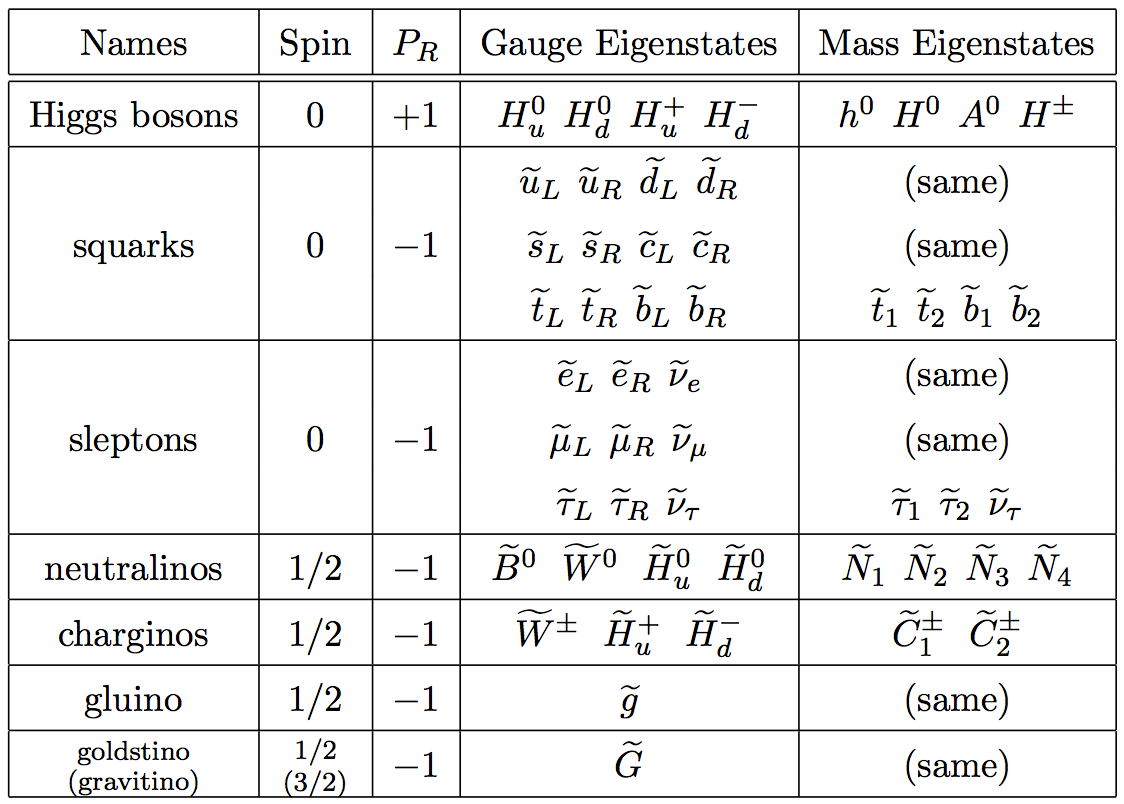
\includegraphics[width=0.75\textwidth]{theory/pics/SUSY_particles_table.png}
		\end{tabular}
		\caption{SUSY particles in MSSM~\protect\cite{Martin:1997ns}}
		\label{fig:SUSY_particles_table}
\end{table}

\FloatBarrier

\subsection{Motivations}

\FloatBarrier

Supersymmetry gives an elegant solution to some of the  previously shown problems which the Standard Model fails to explain. The most important are: 

\begin{itemize}
	\item \textbf{Dark Matter candidate}: The assumption of R-parity conservation prevents the lightest of the SUSY particles, also called LSP, to decay any further into lighter Standard Model particles. In order to fit into the profile of a Dark Matter candidate this particle cannot interact with matter any further, therefore the best choice for the LSP is the lightest neutralino \neutralinoone.  
	
	\item \textbf{Hierarchy problem solution}: the previously mentioned corrections to the Higgs mass are exactly canceled by the symmetric partners of the Standard Model particles with opposite sign. An example of the top quark correction to the Higgs mass being canceled by a supersymmetric scalar top $\widetilde{t}$ correction is shown in \autoref{fig:higgs_loop}.
	
	\begin{figure}[tbh!]
		\centering
		\begin{tabular}{cc}
			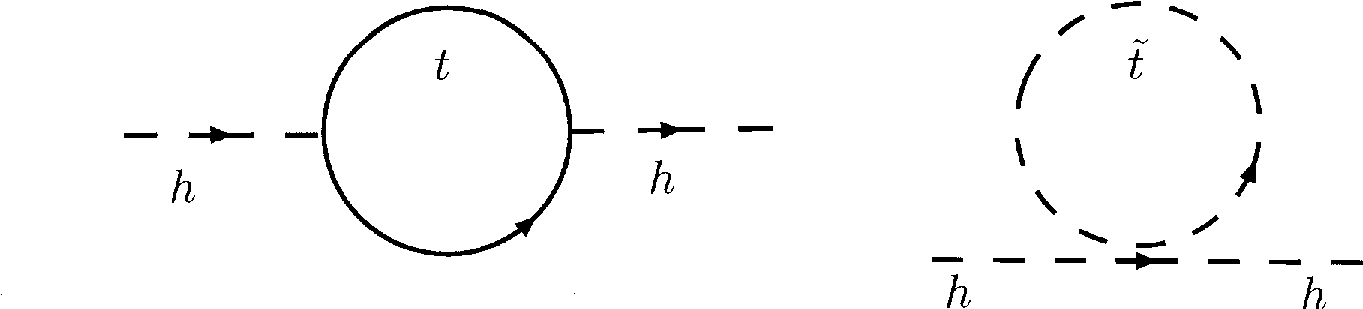
\includegraphics[width=0.75\textwidth]{theory/pics/higgs_loop.png}
		\end{tabular}
		\caption{In SUSY, the correction to Higgs mass by the top quark (left) is inherently cancelled by the contribution from the top quark's supersymmetric partner, the stop (right).}
		\label{fig:higgs_loop}
	\end{figure}

	\item \textbf{Naturalness and parsimony}: Along with the hierarchy problem solution many scientific observations made during the first run of LHC suggest a supersymmetric theory that more naturally explains the weak scale\cite{Craig:2013cxa}. The proposition of a new theory based on the MSSM could also adopt a more "parsimonious" approach. Parsimony involves the inclusion in the theory of additional rules such as assuming there are not additional fields besides the ones required to promote supersymmetry, considering a high SUSY breaking scale, requiring the colored sparticles to be heavier than the uncolored ones, assuming a small number of supersymmetry breaking parameters and finally considering the non-differentiation of the Standard Model generations by the SUSY breaking mechanism. A combination of both naturalness and parsimony leads to sparticles featuring a low mass ($\approx\gev$) stop $\widetilde{t}$, higgsinos $\widetilde{h}$, electroweakinos $\widetilde{W}$ nad sleptons $\widetilde{l}$ and a high mass ($\approx\tev$) gluino $\widetilde{g}$ and squarks $\widetilde{q}$. A summary of the given SUSY particles mass scales is shown on \autoref{fig:SUSY_naturalness}.

	\begin{figure}[tbh!]
		\centering
		\begin{tabular}{cc}
			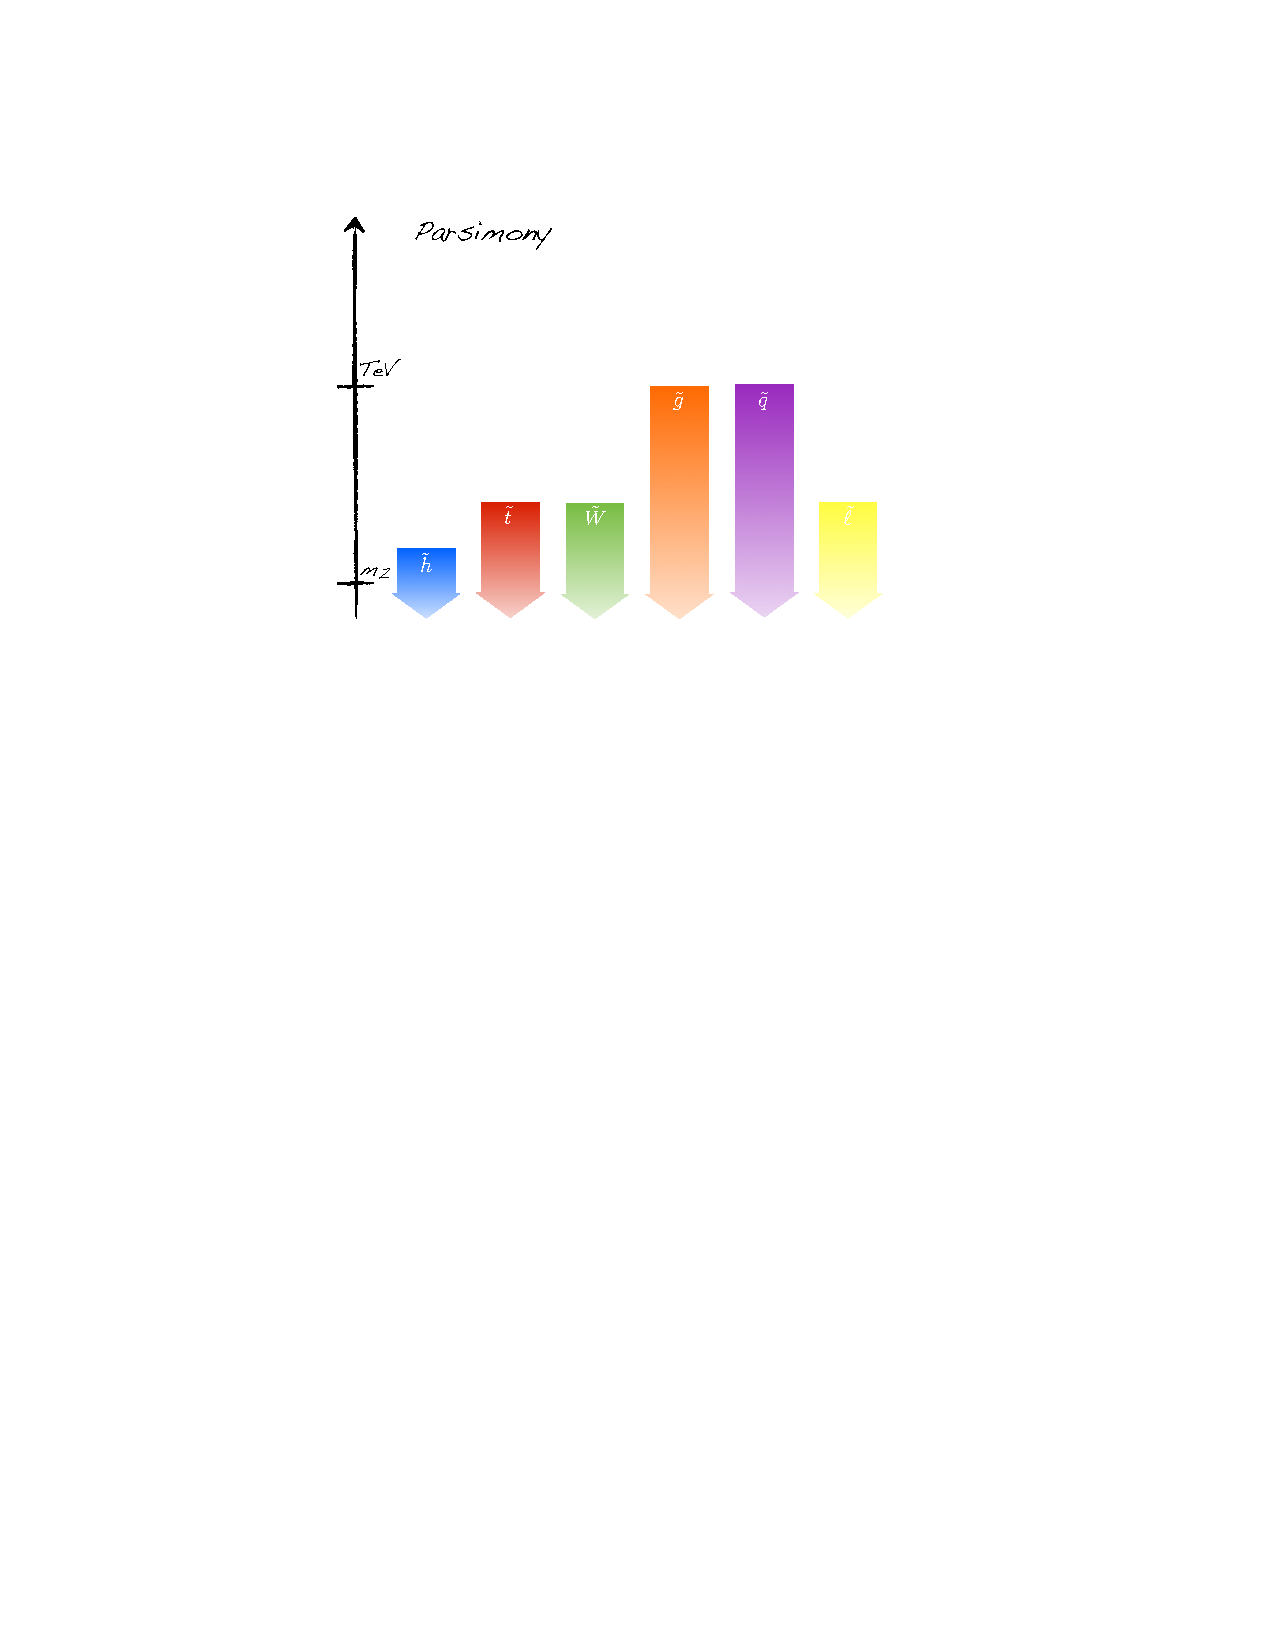
\includegraphics[width=0.75\textwidth]{theory/pics/SUSY_naturalness.pdf}
		\end{tabular}
		\caption{Cartoon illustration of the mass scales for various sparticles dictated solely by electroweak naturalness with sensitivity parameter $\Delta \lesssim 10$\cite{Craig:2013cxa}.}
		\label{fig:SUSY_naturalness}
	\end{figure}
	
	\item \textbf{Gravity and forces unifications}: supersymmetric models , for example minimal supergravity (mSUGRA)\cite{Ellis:2013oxa},can take take into account a gravity-mediated supersymmetry breaking \cite{Martin:1997ns}, leading to unification of the gauge couplings at the GUT scale. Those assumptions further reduce the numbers of MSSM parameters.

\end{itemize}

\FloatBarrier

\subsection{SUSY generic signatures at the LHC with charginos and neutralinos}

\FloatBarrier

The assumptions made by the most important SUSY models set the mass of the first generation charginos \charginopm and next-to-lightest neutralino \neutralinotwo to values not far from the LSP mass \neutralinoone. The possibility of being the first SUSY particles to be discovered puts the spotlight on this topology of SUSY searches in past literature \cite{Abel:2000vs}. 

In case of a mass split between the LSP and next-to-lightest neutralino \neutralinotwo or the lightest chargino \charginopm larger than $\text{M}_{Z}$ or $\text{M}_{W}$, the particles will decay into massive gauge bosons and the LSP \neutralinoone. If not, the decays will occur through virtual gauge boson and scalar fermion exchanges, leading in the final state to the LSP neutralino and a fermion-antifermion pair. It has been realized \cite{Baer:1998bj, Baer:1998sz, Bartl:1999iw, Djouadi:2000aq} that for large values of the parameter \tanbeta, the ratio of the vacuum expectation values of the two doublet Higgs fields which are needed to break the electroweak symmetry in the MSSM, the Yukawa couplings of third generation down-type fermions (b quarks and $\tau$ leptons), which are strongly enhanced, lead to dramatic consequences for the decays of these particles. Indeed, the virtual exchanges of, on the one side, Higgs particles (because the Higgs boson couplings to b quarks and $\tau$ leptons are proportional to \tanbeta) and, on the other side, of third generation down-type sfermions (which tend to be lighter than the other sfermions in this case) become very important.

Many scenarios of those decays has been taken into account considering different SUSY breaking parameters configuration \cite{Djouadi:2001fa}. 

\begin{figure}
	\centering
	\begin{tabular}{cc}
		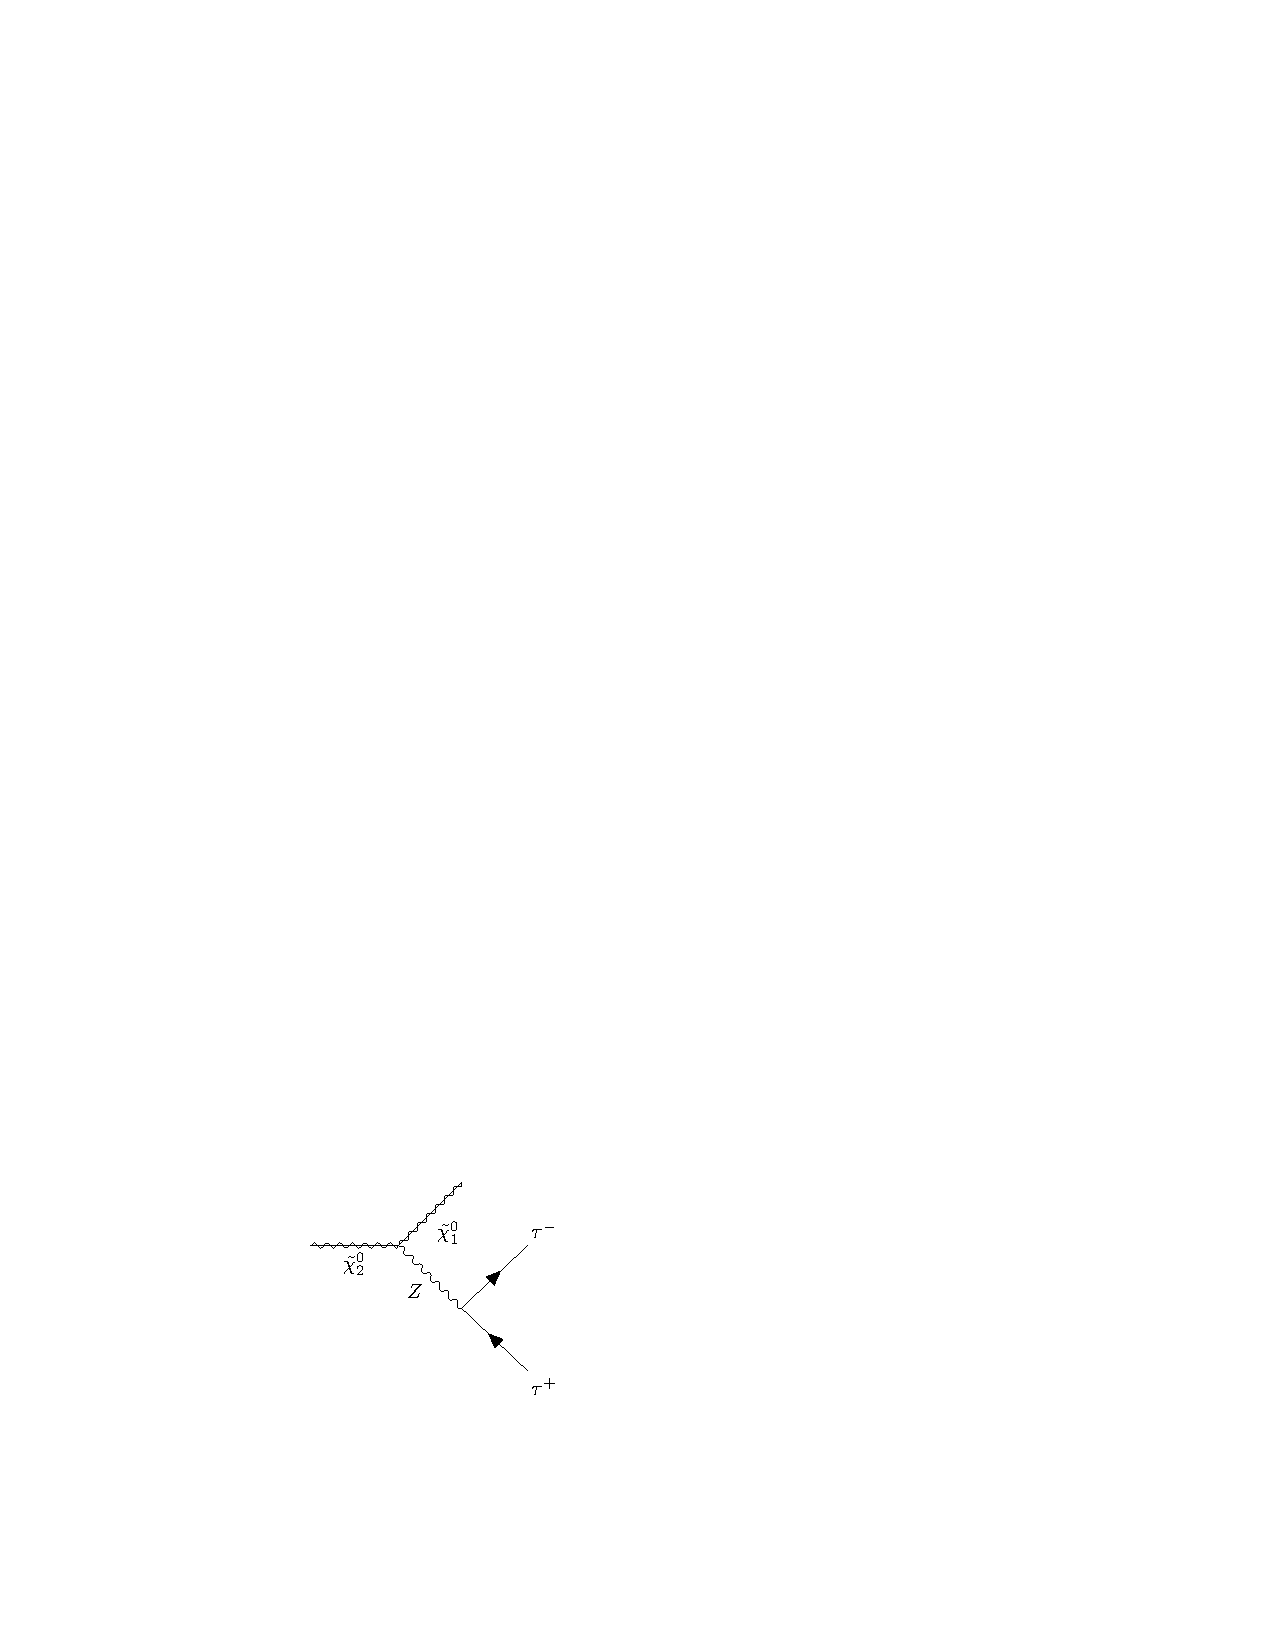
\includegraphics[width=0.40\textwidth]{theory/pics/chi02_tautau.pdf}
		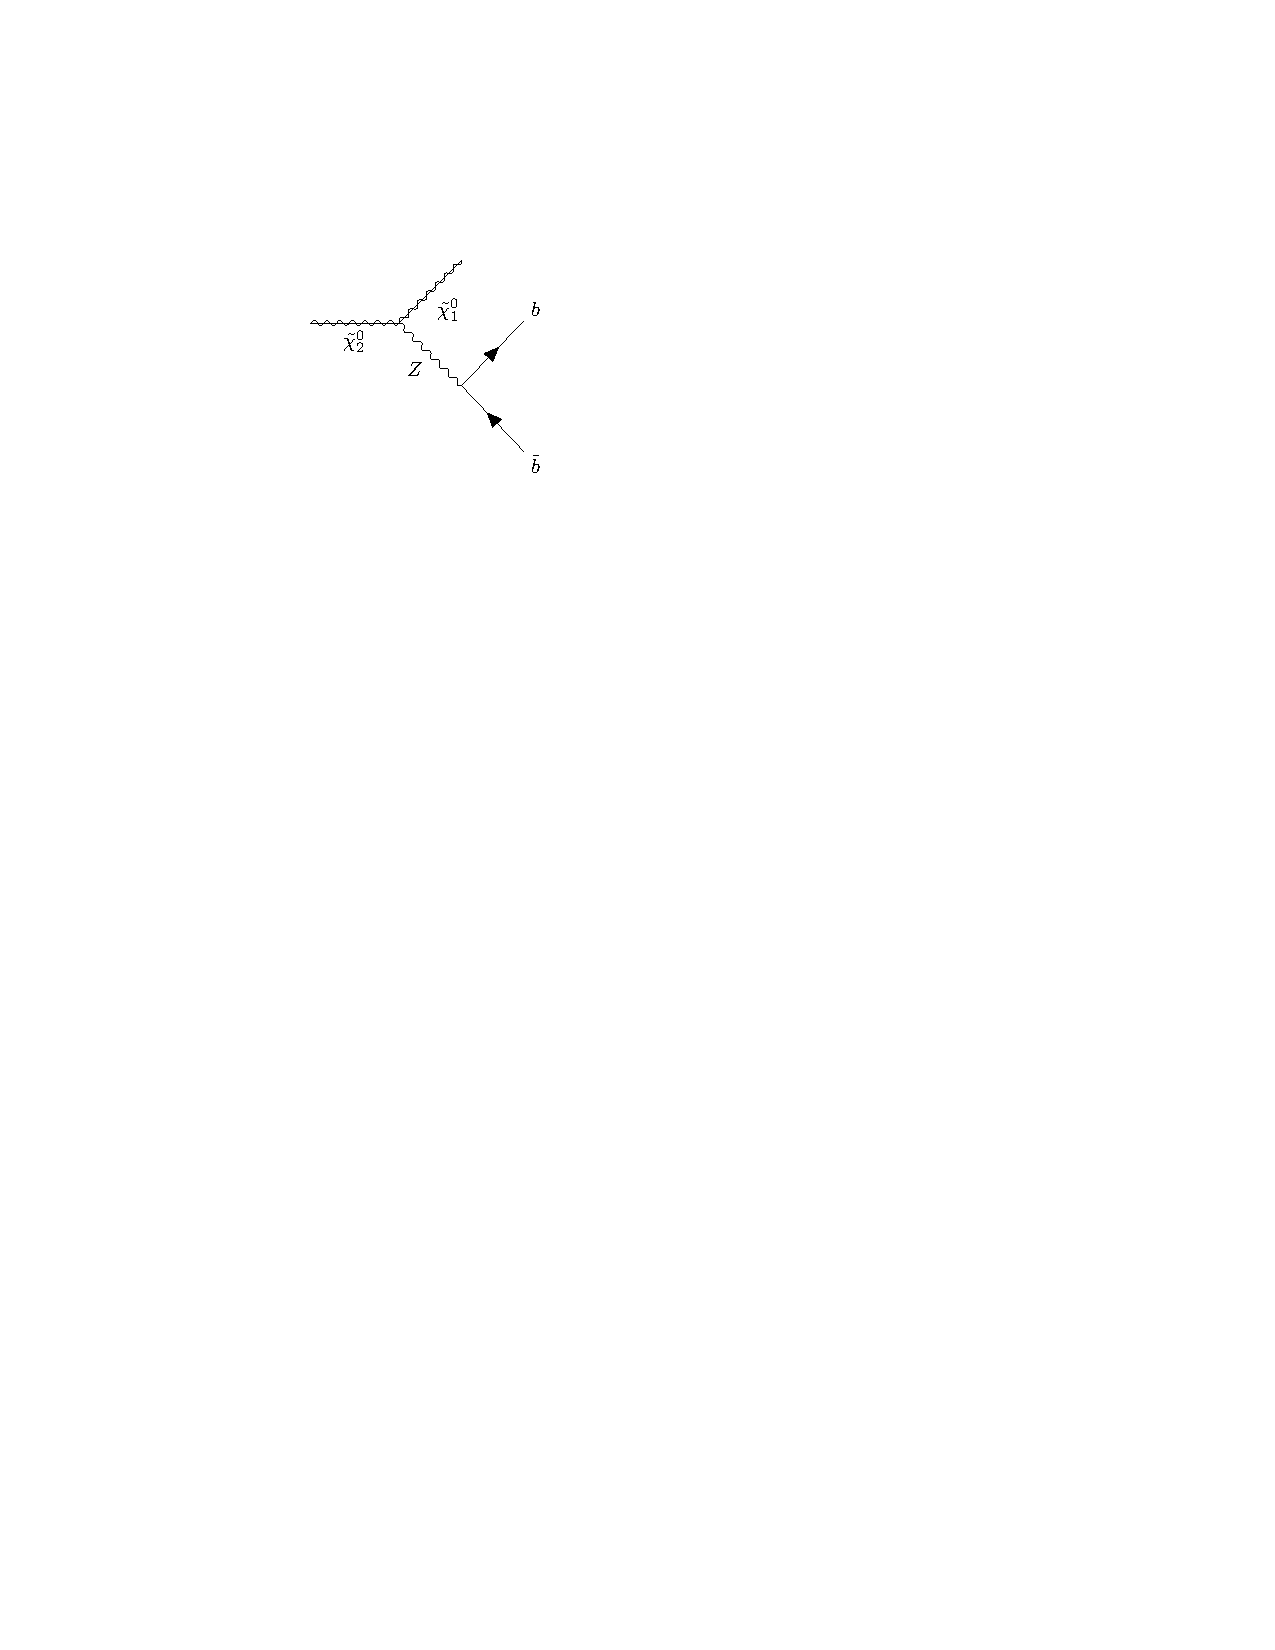
\includegraphics[width=0.40\textwidth]{theory/pics/chi02_bbarb.pdf}
	\end{tabular}
	\caption{The Feynman diagrams contributing to the three-body decays of charginos and neutralinos into the LSP and two fermions}
	\label{fig:SUSY_3bodydecay_chi}
\end{figure}

For example \autoref{fig:SUSY_3bodydecay_chi} shows a couple of the possible Feyman diagrams of $\neutralinotwo \longrightarrow \neutralinoone\tau^{+}\tau^{-}$ and $\neutralinotwo \longrightarrow \neutralinoone b \bar{b}$. \autoref{fig:br_chitautau} and \autoref{fig:br_chibbarb} show, respectively, the branching ratios $\text{BR}(\neutralinotwo \longrightarrow \neutralinoone\tau^{+}\tau^{-} )$ and $\text{BR}(\neutralinotwo \longrightarrow \neutralinoone b \bar{b})$, as functions of $m_{\widetilde{\tau}1}$ or $m_{\widetilde{b}1}$ for $\mu = 500\gev$ (a), as a function of $\mu$ (b) and as a function of \tanbeta (c) for $m_{0} = 300\gev$. There is an evident competition between $b\bar{b}$ and $\tau^{+}\tau^{-}$ final states. In the case of a light A boson and for large \tanbeta values, the A and h contributions are much more important in the decay $\neutralinotwo \longrightarrow \neutralinoone b \bar{b}$ than in the channel $\neutralinotwo \longrightarrow \neutralinoone\tau^{+}\tau^{-} $ because of the larger b-quark mass and the color factor; the Higgs contribution makes then $\text{BR}(\neutralinotwo \longrightarrow \neutralinoone b \bar{b})$ dominating, except when $\widetilde{\tau}_{1}$ is very light, and the two body decay $\neutralinotwo \longrightarrow \stau \tau$ is close to occur, making $\text{BR}(\neutralinotwo \longrightarrow \neutralinoone\tau^{+}\tau^{-} )$ close to unity. Even for heavy A, and H bosons, $\text{BR}(\neutralinotwo \longrightarrow \neutralinoone b \bar{b})$ can reach the level of 50\%. However, for large enough values of \tanbeta and $\mu$, it is the decay channel $\neutralinotwo \longrightarrow \neutralinoone\tau^{+}\tau^{-} $ which dominates, since the stau is always lighter than the $\widetilde{b}_{1}$ state and its virtual contribution is larger, despite of the color factor. The sum of the two branching ratios is in general close to unity.

\begin{figure}[tbh!]
	\centering
	\begin{tabular}{cc}
		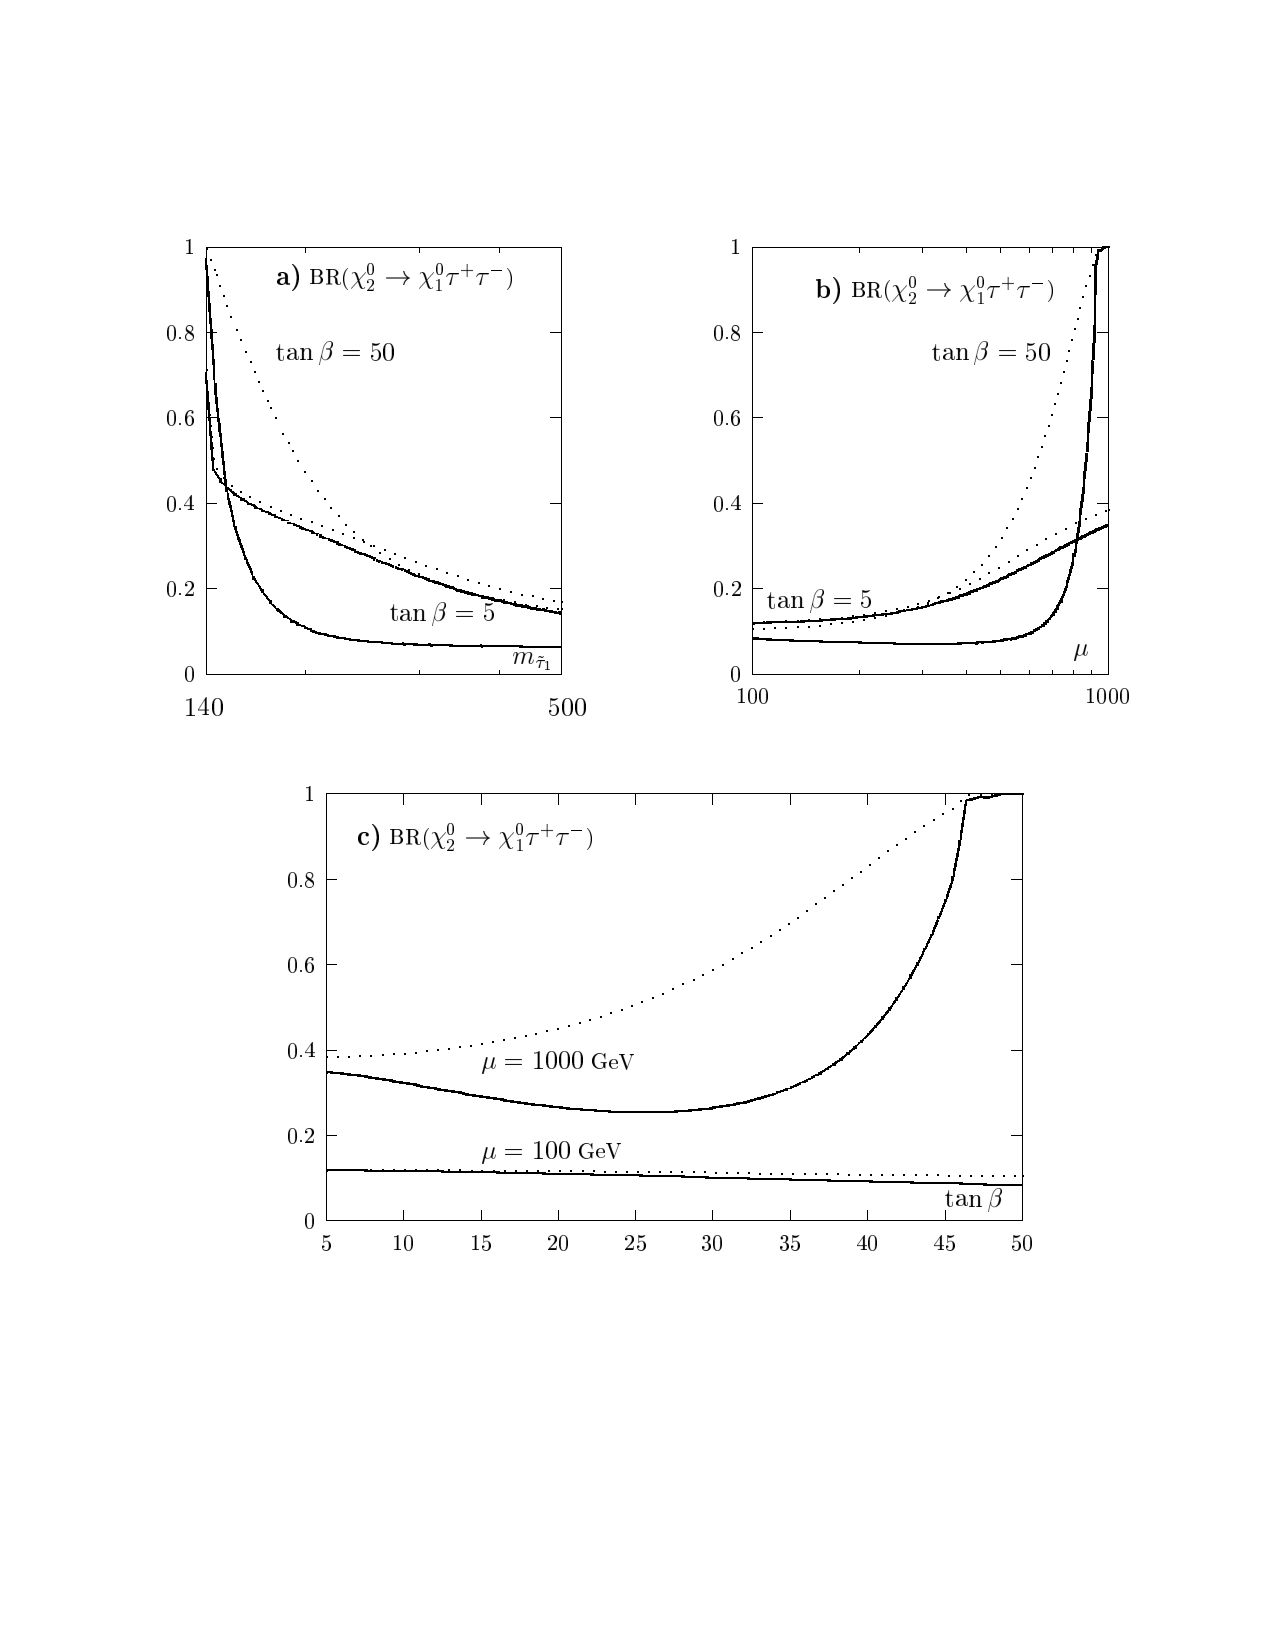
\includegraphics[width=0.80\textwidth]{theory/pics/br_chitautau.pdf}
	\end{tabular}
	\caption{The branching ratio $\text{BR}(\neutralinotwo \longrightarrow \neutralinoone\tau^{+}\tau^{-} )$ for two values of \tanbeta = 5 and 50 and two values of $M_{A} = 100\gev$ (dashed lines) and 500\gev (solid lines) as a function of $m_{\widetilde{\tau}1}$  for $\mu = 500\gev$ (a) as a function of $\mu$ assuming $m_{0} = 300\gev$ (b) and as a functionof \tanbeta for two values of $\mu = 100$ and $1000\gev$ (c); $M_{2}$ is fixed to $150\gev$\cite{Djouadi:2001fa}.}
	\label{fig:br_chitautau}
	
\end{figure}

\begin{figure}[tbh!]
	\centering
	\begin{tabular}{cc}
		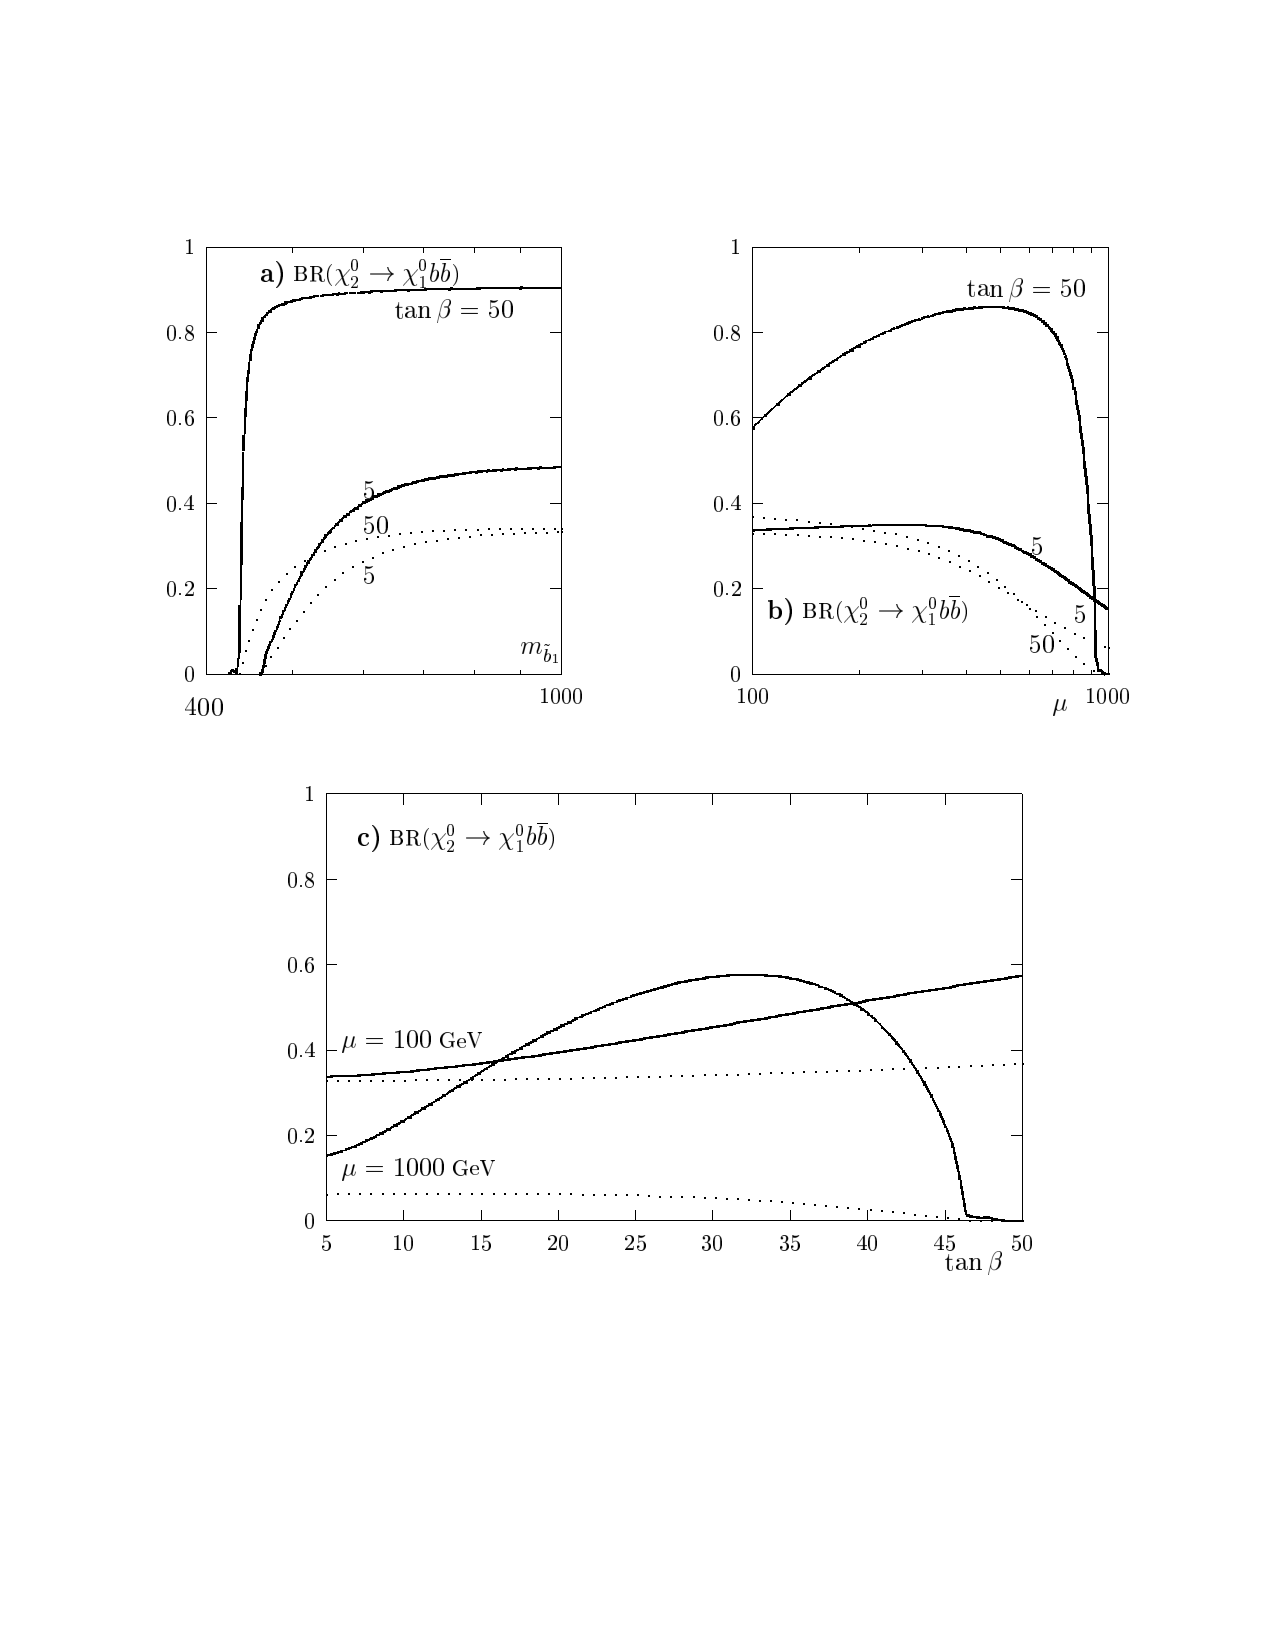
\includegraphics[width=0.90\textwidth]{theory/pics/br_chibbarb.pdf}
	\end{tabular}
	\caption{The branching ratio $\text{BR}(\neutralinotwo \longrightarrow \neutralinoone b \bar{b})$ for two values of $\tanbeta = 5$ and $50$ and two values of $M_{A} = 100\gev$ (solid lines) and $500\gev$ (dashed lines) as a function of $m_{\widetilde{b}1}$ for $\mu = 500\gev $ (a) as a function of $\mu$ assuming $m_{0} = 300\gev$ (b) and as a function of \tanbeta for two values of $\mu = 100$ and $1000\gev$ (c); $M_{2}$ is fixed to $150\gev$\cite{Djouadi:2001fa}.}
	\label{fig:br_chibbarb}
	\end{figure}

\FloatBarrier

\clearpage
